\documentclass[a4paper,twoside]{article}
\usepackage[utf8]{inputenc}
\usepackage{wrapfig}
\usepackage{subcaption}
\usepackage{amsmath,amsthm,array} 
\usepackage{multicol}
\usepackage{adjustbox}
\usepackage{multirow}
\usepackage{longtable}
\usepackage{gensymb}
\usepackage{supertabular}
\usepackage{url}
\usepackage{graphicx}
\usepackage{lipsum}
\usepackage[english]{babel}
\usepackage{fancyhdr}
\usepackage{caption}
\usepackage{blindtext}
\usepackage{lastpage}
\usepackage[resetfonts]{cmap}
\usepackage{fancyvrb}
\begin{VerbatimOut}{ot1.cmap}
%!PS-Adobe-3.0 Resource-CMap
%%DocumentNeededResources: ProcSet (CIDInit)
%%IncludeResource: ProcSet (CIDInit)
%%BeginResource: CMap (TeX-OT1-0)
%%Title: (TeX-OT1-0 TeX OT1 0)
%%Version: 1.000
%%EndComments
/CIDInit /ProcSet findresource begin
12 dict begin
begincmap
/CIDSystemInfo
<< /Registry (TeX)
/Ordering (OT1)
/Supplement 0
>> def
/CMapName /TeX-OT1-0 def
/CMapType 2 def
1 begincodespacerange
<00> <7F>
endcodespacerange
8 beginbfrange
<00> <01> <0000>
<09> <0A> <0000>
<23> <26> <0000>
<28> <3B> <0000>
<3F> <5B> <0000>
<5D> <5E> <0000>
<61> <7A> <0000>
<7B> <7C> <0000>
endbfrange
40 beginbfchar
<02> <0000>
<03> <0000>
<04> <0000>
<05> <0000>
<06> <0000>
<07> <0000>
<08> <0000>
<0B> <0000>
<0C> <0000>
<0D> <0000>
<0E> <0000>
<0F> <0000>
<10> <0000>
<11> <0000>
<12> <0000>
<13> <0000>
<14> <0000>
<15> <0000>
<16> <0000>
<17> <0000>
<18> <0000>
<19> <0000>
<1A> <0000>
<1B> <0000>
<1C> <0000>
<1D> <0000>
<1E> <0000>
<1F> <0000>
<21> <0000>
<22> <0000>
<27> <0000>
<3C> <0000>
<3D> <0000>
<3E> <0000>
<5C> <0000>
<5F> <0000>
<60> <0000>
<7D> <0000>
<7E> <0000>
<7F> <0000>
endbfchar
endcmap
CMapName currentdict /CMap defineresource pop
end
end
%%EndResource
%%EOF
\end{VerbatimOut}
\usepackage[margin=0.7in]{geometry}
\numberwithin{equation}{section}
\pagestyle{fancy}
\fancyhf{}
\rhead{Ankush B}
\lhead{Basics of Astronomy}
\cfoot{\thepage-\pageref{LastPage}}
\newcommand\sun{\cdot}
\title{Basics of Astronomy}
\author{Ankush Banerjee}
\begin{document}
\maketitle
\tableofcontents
\newpage
\section{Disclaimer}
\paragraph{}
The main intention of this document is to serve as a rough guide book for the volunteers for their reference in the field. The structure of this document is made in a way that it addresses few of the questions the volunteer would most likely encounter during a typical outreach session. This will always remain a work in progress hence please mail me your suggestions at ankushabanerjee@gmail.com. Also do check out the references for further reading (I have quoted some Wikipedia articles when I couldn't find more compelling evidence of the same, feel free to suggest some better sources). Also note that I have skipped many details which are mentioned in the citations, so please do go through those whenever possible.
\section{Questions relevant to astronomy.}
\paragraph{}
A small disclaimer that one might have to keep in mind before we start would be to understand that astronomy is a huge field of study. This originated when the scientific method met astrology. Astronomy has several branches, some of them being, astrophysics, astrochemistry, astrobiology, astrometry etc. We would get into these topics soon.
\subsection{How did astronomy begin?}
\paragraph{}
This might not be one of the most common questions that one might get asked, however, it is important to understand the origin of astronomy. Also, this would be a two part question since one of them addresses, roughly, how did we arrive to the helio-centric model and the other would briefly touch on who were the notable scientists who contributed to the modern day astronomy.
\subsubsection{How did we arrive to the Helio-centric model?}
\paragraph{}
Our curiosity of the heavens above have been present since the dawn of times. Since our exodus form Africa, when we needed some guidance to navigate through the unknown lands, and know the directions and essentially know our place in this world, we looked up at the heavens as our guides. Fast forward a few thousand years, when we became settlers, and we discovered agriculture, we were able to devote much more time to look up at the heavens and come up with elaborate stories to connect the dots of light together. This helped us keep our crops healthy, know when to harvest, when to plant the seeds, etc. Knowing these patterns was vital to our survival. Hence few of the early civilizations came up with their own versions of astronomy which they used to map the skies. The most well documented ones however were the Arabic astronomers. The name they gave to most of the heavenly lights (which we now know to be stars) are the same that we use today. 
\paragraph{}
Apart from documenting and naming the stars, they also noticed that there were some bodies that did not move in accordance with it's neighbors. These were considered rulers of the heavens by some, and by others as wanderers/wandering stars (planetai in ancient greek, read this article from space.com about the word's origin \cite{Planets_1}). This was also the time when Earth was considered to be the center of the universe and there were only a few that thought that the earth was a sphere (which first came from Plato without much ambiguity, refer  \cite{wiki_planet_round}). This around the time when Aristotelian (Aristotle being one of Plato's student) astronomy placed the spherical earth on the center of the universe and all other planets went around it, controlled by some unknown force that permeated through everything. This was quickly absorbed by the church at that time since this model of the cosmos left enough space for the creator to determine the motion of the heavens.
\paragraph{}
This model of the universe was not openly contested for a long time until Nicolas Copernicus in 1543 (also the year he was crucified for doing so) challenged the Aristotelian view of the cosmos by suggesting a helio-centric model of the universe (mind you, he said the sun was the center of the cosmos). Then came Galileo Galilei, who was the first person to use a telescope to look at the planets, and in particular the moons of Jupiter to further push the idea of a helio-centric model since the Aristotelian model did not incorporate planets having bodies rotating around them. This  was one of the pivotal moments of the Renaissance era that led to the modern astronomy, and led to the differentiation of astronomy and astrology. The book 'On the Shoulders of Giants: the Great Works of Physics and Astronomy' \cite{OTSOG} is a must read if one wishes to go through the nuances of their works and get a deeper understanding of how did they arrive at their conclusions. 

\subsubsection{How did we know that the sun is a star?}
\paragraph{}
\textbf{Note:} This answer is heavily influenced by \cite{AASP}, so do give it a read.
\paragraph{}
As mentioned in the previous section, for most of our history we considered ourselves to be at the center of a huge celestial sphere with the stars being stuck to the inside of the sphere. The heavenly bodies such as the planet, moon and the sun were thought to move in between the inner surface of this sphere and the earth. However, our journey of the sun being classified as a star took thousands of years and a lot of people and their work. 
\paragraph{}
The first person to have suggested the same was \textbf{Anaxagoras} in 450 BC, who thought that the sun and stars were fiery stones that gave out heat, however, the stars were too far away for their heat to be felt. However his ideas were met with disapproval since it did not fit the ideas of the time. 
\paragraph{}
Next was \textbf{Aristarchus of Samos} (Samos being an island in the Aegean sea) who tried to measure the size of the sun, and though his measurements were inaccurate, he was able to conclude that the sun was much larger than the earth. He then suggested that the Earth orbits around the sun rather than the other way around. He also suggested that the stars were nothing but distant suns. However, since Anaxagoras and Aristarchus lacked the means to observe the sizes of, or the distance to the stars and hence had no proof for their ideas and hence were forgotten. 
\paragraph{}
Then came \textbf{Claudius Ptolemaeus} (Ptolemy) of Alexandria, who in 140 AD suggested the geocentric model of the universe and clubbed the sun in with the planets rather than with the stars. This idea model was not challenged for the next 14 centuries mostly because this model was endorsed by the catholic church which was very powerful at that time. 
\paragraph{}
However things changed around the 15$^{th}$ century when Mikolaj Kopernik (known as Nicholas Copernicus outside of his native Poland), published the book \textbf{De revolutionibus orbium celestium} where he challenged the ideas of a geocentric universe with the presence of a helio-centric universe. Even if it was simple, the copernican model set sun apart from the planets, but did not mention anything about the stars and their relation to the sun. Copernicus waited for quite some time before publishing his work in 1543, the year he was crucified. 
\paragraph{}
Then came \textbf{Giordano Bruno} in the late 16th century, who suggested that if the earth was a planet like all others then it would not make sense to divide the universe into a sphere of fixed stars and a solar system. He proposed that the sun is a star as well, and that the universe is infinitely large, and that there were possibly many other worlds like ours out there around the stars. 
\paragraph{}
Next was \textbf{Galileo Galilei}, an Italian scientist, who lived from 1564 to 1642. He was the first person who used the newly invented telescope to look up at the stars and planets, he discovered the satellites of Jupiter with which he was able to reinforce the Copernican principle of a helio-centric universe and was able to also conclude that the stars must be very far away from the earth since they appeared as point sources even through the telescope. However, at that time, Galileo, Bruno, and Copernicus had no evidence at that time the sun was the same as the stars since they had no means of proving the same. 
\paragraph{}
At the same time as Galileo, \textbf{Johannes Kepler} (Germany, 1571 to 1630 AD), studied the positions of the planet and determined the three laws planetary motion that firmly put the sun in the center of the the solar system, with the planets orbiting the sun.
\paragraph{}
A century later, \textbf{Christiaan Huygens} (Holland circa 1650 AD) determined the distance to the star Sirius assuming that the star was as bright as the sun and appeared faint only because it was very far away. He found that the distance to Sirius must be very great. At this time, then, the idea that the Sun is a star was considered seriously by scientists.
\paragraph{}
Then a few years later, Issac Newton, in 1665 realized that it was gravity that held the solar system together. (Just a side note, the story of Newton getting the idea of gravity by looking at an apple and the moon is mostly a dramatization by Voltaire, there are no records of it actually happening). Newton then determined the formula that describes how gravity works and showed that this explains the orbits and motion of the planets around the Sun and of moons around planets, and therefore also Kepler's three Laws of planetary motion. The motion of the planets and moons were now explained by a single formula: Newton's Law of Gravity. People speculated that this same law might be valid all through the universe.
\paragraph{}
Finally, in 1838, \textbf{Friedrich Bessel} was the first astronomer to reliably determine the values of distance from the sun to another star by the method of parallax, without any of prior assumptions about nature of the stars. Distances to other stars followed soon, and then people could calculate the true brightness of stars, correct for their distance to us, and find them to be about as bright as the Sun. When other things about the Sun were also found to be like those of stars, such as its surface temperature and chemical composition, using spectroscopy (which was a well known activity by that time), then the proof was finally here that the Sun is a star.
\subsubsection{How did we come about astronomical spectroscopy, and why do we care?}
\paragraph{}
This answer is heavily influenced by \cite{ASHistory}, do go through the website for further references. 
\paragraph{}
Astronomical spectroscopy was an offshoot of the chemist's attempts to analyze materials on earth as well as scientist' interest in the nature of color. Circa 1850 Joseph Fraunhofer mounted a prism in front of the objective lens of a telescope making a crude spectroscope. Fraunhofer was an optician and was able to make prisms that were pure and hence did not absorb much of the light went into them. He found that when light from the sun and bright stars like Sirius was analyzed there were characteristic absorption lines present in the spectrum produced. However, Fraunhofer died before he could study this phenomena fully. 
\paragraph{}
A major advance was made in 1859 by Gustav Kirchhoff and Robert Bunsen (the Bunsen burner guy). Bunsen's development of a powerful gas burner was essential for the research they did when they heated certain elements and it started emitting lines at the same spot as the black lines in the solar spectrum. That is, they identified the cause of the dark lines in the solar spectrum. They discovered that the bright lines were coming from hot gas, whereas the dark lines were because of the absorption of light due to cooler gas above the sun's surface. 
\paragraph{}
They found that every chemical element produces a distinct spectrum. This provided a sort of "fingerprint" of the element in the gas cloud. Throughout the 1860s Kirchhoff was able to identify some 16 elements distinctly, in the mess of hundreds of lines he saw in the solar spectrum. From those data Kirchhoff was able to speculate the sun's composition and structure. 
\paragraph{}
Since these advancements, scientists like William Huggins and Angelo Secchi gathered as much data as possible, and like the other scientists of their age, started classifying the data into certain schemes. Three basic groups emerged, blue and white stars, yellow stars (sun like stars), and red stars. Later, in 1885, Edward C. Pickering at the Harvard College Observatory undertook an ambitious program to classify the stars using data recorded in photographic plates. By 1890 over 10,000 stars had been prepared that grouped them into thirteen spectral types. Following Pickering's vision, Annie Jump Cannon expanded the catalog to nine volumes and over a quarter of a million stars by 1924 and developed a system of ten spectral types - \textbf{O, B, A, F, G, K, M, R, N, S} - that astronomers accepted for world-wide use in 1922. 
\paragraph{}
However, one thing to note would be that since the discovery of this new technique of spectroscopy, a big disadvantage was soon discovered when dim objects were considered. That is, the prism technique of dispersing the light meant that most of the signal would be lost (either by scattering within the glass, or by absorption by the glass medium). The alternative to achieving the same effects would be to use the diffraction grating which is essentially a surface made out of several equidistant lines that help breaking the light into a spectrum. 
\paragraph{}
\textbf{Henry A. Rowland}, an American physicist at Johns Hopkins University, was the person most responsible for making the larger and more accurate diffraction gratings that revolutionized spectroscopy in the 1880s. This technology helped him achieve as many as 43000 lines per inch, twice as large as achieved earlier. 
\paragraph{}
Another instrument that came into use around this time was the \textbf{spectro-heliograph} that gave an image of the entire solar disk in one particular wavelength. While it's invention was given to \textbf{George Ellery Hale} (the same person who played a pivotal role in setting up mount Wilson observatory) in 1889, earlier versions of the tool had been around since 1870. This tool helped researchers to see the sun in several different wavelengths and hence brought out several different features of the sun which helped researchers study this body in much more detail. He was also able to use his stunning results to eloquently argue that stellar and solar research complemented each other and that research on the nearest star to us would help scientists understand the secrets of all other stars. 

\subsubsection{What are constellations, what are their origins and why are they relevant?}
\paragraph{}The word constellation comes from the Latin term cōnstellātiō  and is a result of humans being great at recognizing patterns (kind-of the reason why proper graphs are help us visualize the data and understand the nature of the data). This is something that helped us survive nature throughout the ages. This was presumably the same thing that led our ancestors to look up at the skies and make out patterns (which are heavily influenced by their location and their daily experiences) by connecting the dots (stars). The practice might've started as a need to track time (at night) and seasons which, with the advent of agriculture, became crucial for the survival of our civilizations, before the calendar was invented. The wiki definition of a constellation would be a "set of stars" (refer \cite{wiki_constellation} for further details). I would recommend that one could go through the Wikipedia page for constellations to get a deeper understanding of the history of how they came to be. 
\paragraph{}
Since every major civilizations came up with their own different stories, they had different constellations. However, to avoid confusion we would be using the constellations set by the International Astronomical Union (IAU) in the future. As per their list, there are 88 modern constellations, out of which 48 are listed by Ptolemy in his Almagest in the second century (ref. \cite{wiki_constellation}), which were built upon by \textbf{Petrus Plancius (1592, 1597/98 and 1613)}, \textbf{Johannes Hevelius (1690)} and \textbf{Nicolas Louis de Lacaille (1763)} who named 14 constellations and renamed a fifteenth one. In 1922, \textbf{Henry Norris Russell} aided the IAU (International Astronomical Union) in dividing the celestial sphere into 88 official constellations. Prior to this, Ptolemy's list of 48 constellations with many additions made by European astronomers had prevailed. However, these divisions did not have clear borders between them. It was only in 1930 that \textbf{Eugene Delporte}, the Belgian astronomer created an authoritative map demarcating the areas of sky under different constellations.
\paragraph{}
The aim of this system is area-mapping, that is, the division of the celestial sphere into  contiguous fields. Out of the 88 modern constellations, 36 lie predominantly in the northern sky, and the other 52 lie in the southern. 
\paragraph{}
Coming to their relevance. In the past, the constellations were used to notify the locations of the stars/objects within a constellation. And the convention of naming the stars with their brightness was used. However, as technology advanced, we kept mapping an increasing number of stars otherwise invisible to the naked eye. This made the old naming convention obsolete and hence catalogue names were given to every object. Hence these days, astronomers have seemingly abandoned the usage of constellation names, and are using the catalogue names instead, or just their coordinates in the celestial sphere. 

\subsection{What are the coordinate systems?}
\paragraph{}
You're an astronomer, and you have discovered a very interesting source in the sky and you need to tell the community about your discovery. The first step to this would be to tell them it's location in the sky. The art (yes, it's an art) of finding the exact location of an object in the sky is called \textbf{astrometry}. It is one of the most important things in astronomy, and hence has it's own field of study. However, before we can dive into astrometry, you need to know what are the systems available to you and which ones should you use and how. The following would be a brief run down (without much of it's history) of the available systems. I would highly recommend that you go through these and go through the page cited in \cite{astrometry_wiki}. 
\subsubsection{Altazimuth Coordinate system}
\begin{wrapfigure}{l}{0.5\textwidth}
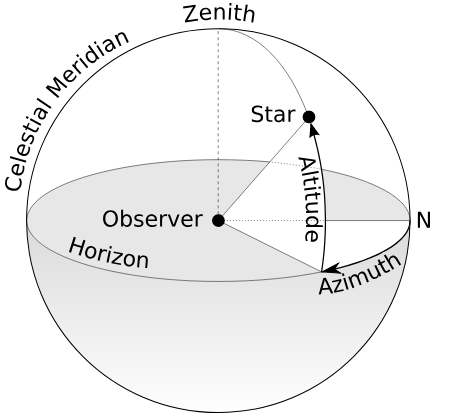
\includegraphics[width=0.9\linewidth]{fig1.png} 
\caption{Altitude and Azimuth measurement \\ Image source \cite{azimuth_wiki}}
\label{fig1}
\end{wrapfigure}
\paragraph{}
The name, Altazimuth is actually the combination of the two axes, namely \textbf{Altitude} and \textbf{Azimuth}. The altitude angle is the angle that says how high the object is in the sky from the horizon. So with this definition, the point right above our head will be at 90$\degree$ altitude. This point is called the \textbf{zenith}. The horizon is at 0$\degree$ altitude, and anything in between that is above the horizon is from 0$\degree$ to +90$\degree$. Also, the point right below us, called the \textbf{Nadir} is at -90$\degree$. Sometimes the zenith is used instead of altitude angle, and hence is referred to as the \textbf{zenith angle}, which is basically a complement to the altitude angle. The other angle that helps pin point the object at a certain location, at a given time, is the Azimuth angle. To get this we first join the north and south poles, and then the angle moving from north-east-south-west-north is the azimuth angle. This might be a bit ambiguous, but then the figure \ref{fig1} should clear things out. Hence, to put things into perspective, north to east is 90$\degree$ azimuth, north-east-south is 180$\degree$ azimuth, and north-east-south-west is 270$\degree$ azimuth. North to north would be 360$\degree$. The reverse gives us degrees in negatives. 
\paragraph{}
Now, a few things that one would have to keep in mind is the radius of the sphere in figure \ref{fig1}, is 5 Km, hence if we have a radius of greater than 5 Km then the curvature of the earth would skew the altitude measurements. This also means that this coordinate system is highly location specific. Also, since the earth rotates, the coordinates of any object changes through the night, and hence when communicating the location of any event in the sky, we would have to give our location of observation, the time of observation and the location of the object in the sky during that time. This obviously is too much work, and hence is prone to errors. To avoid these and many other issues, the equatorial coordinate system is used. To know more about azimuth, read through it's wiki page \cite{azimuth_wiki} and \cite{coord_wiki}.
\subsubsection{Equatorial Coordinate system}
\begin{wrapfigure}{l}{0.5\textwidth}
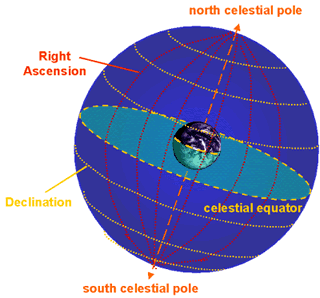
\includegraphics[width=0.9\linewidth]{fig2.png} 
\caption{Equitorial Coordinate system \\ Image source \cite{equi_coord1}}
\label{fig2}
\end{wrapfigure}
\paragraph{}
Now, we know the latitudes and longitudes on earth, and how they form a grid. The equatorial coordinate system is just the projection of this coordinate system into the celestial sphere. Hence \textbf{latitude becomes declination and longitude becomes right ascension}. This kind of coordinate system has the celestial north pole set as the north, that is, as shown in the figure \ref{fig2}. 
\paragraph{}
Now, one might notice that the declination can be easily calculated since that is essentially how high the source is from the celestial equator (which is essentially a projection of the equator on the celestial sphere). However, in order to find the right ascension we need a reference celestial longitude which would be 0 hour. The line we use as a reference is the \textbf{vernal equinox} which is considered to be at 0 hour. 
\paragraph{}
Now, one might be confused as to what do I mean by \textbf{vernal equinox}, how did I get that line, are there any other points of importance in the celestial sphere? The answer to all those questions is yes. Now, before we get into vernal equinox, and what it signifies we need to modify the figure \ref{fig2} a bit. Now, one might know that there is a tilt in the earth's axis, (of roughly \textbf{23.5$\degree$}). This tilt causes the sun's light to fall on earth differently throughout the day, meaning when the southern hemisphere is towards the sun, the northern hemisphere undergoes shorter days, and longer nights, that is winter season (imagine the earth rotating all the while being tilted and the sun's light coming from the left). The opposite happens in case of the southern hemisphere, that is, it has longer days, and shorter nights, in short summer season.
\begin{wrapfigure}{r}{0.5\textwidth}
\begin{center}
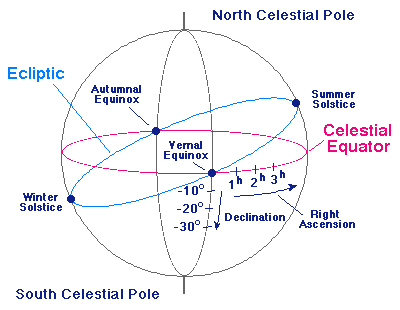
\includegraphics[width=0.8\linewidth]{fig3.png} 
\caption{Equatorial coordinate system with ecliptic \\ Image source \cite{equi_coord2}}
\label{fig3}
\end{center}
\end{wrapfigure}
\paragraph{}
Now, given that the earth rotates, we have the light from the sun rotating through this tilt. Hence, when we started off this explanation, we considered the sun's light from the left, now we move the earth to the opposite part of it's orbit so that we have the sun light coming from the right of figure \ref{fig2}. This is when the northern hemisphere has summer season, and the southern hemisphere has winter at a given time of a year.
\paragraph{}
Now, if we map this position of the sun throughout the year, into the celestial sphere, we get the line called the \textbf{ecliptic}. Refer the figure \ref{fig3}. Now, we see that once we map this, we have two points that intersects with the celestial equator. These points of intersection are those where the day and night are equal (no matter where you are on earth). These points of equal days and nights are called equinoxes. 
\newpage
\clearpage
\paragraph{}
There are two equinoxes, namely, \textbf{vernal equinox} (the time of the year being \textbf{21$^{st}$ March}) when the sun is traveling from southern hemisphere of the celestial sphere to the northern hemisphere, and, \textbf{autumnal equinox} (the time of the year being \textbf{22$^{nd}$ September}) when the sun is traveling from northern hemisphere of the celestial sphere to the southern hemisphere. 
\paragraph{}
Since the sun travels to the northern hemisphere in March, one can say that vernal equinox marks the beginning of the summer season in the northern hemisphere. And when it exits the northern hemisphere in September, it marks the beginning of the winter season for the northern hemisphere.
\paragraph{}
Now, the other two extremes, as shown in figure \ref{fig3}, are the Solstices, that is, the \textbf{winter and the summer solstices}. These points are the points of extremities in the path of the sun through the sky. These are those periods of the year when the day and light length are at the extremes. The \textbf{winter solstice (22$^{nd}$ December)} is that day in the northern hemisphere that has the shortest day and the longest night. The opposite is true for \textbf{summer solstice (21$^{st}$ June)} when, in the northern hemisphere, the day is the longest. 
\paragraph{NOTE: The equatorial coordinate system is the standard system}
\subsubsection{Ecliptic coordinate system}
\paragraph{}
Now, another similar, but not so widely used, coordinate system is the ecliptic coordinate system that considers the ecliptic as the fundamental plane (equator). The poles become the ecliptic poles and declination becomes ecliptic latitude and right ascension becomes ecliptic longitude. One can go through their wiki page for further details. However, one thing that remains constant is the role of vernal equinox in deciding 0 hours for both the systems.
\subsubsection{Galactic coordinate system}
\paragraph{}
This is the coordinate system that takes the galactic plane as the fundamental plane. This is sometimes used when one wants to map the distribution of globular clusters (we will come to those later) around our galaxy, or when someone wants to plot the locations of the nearby galaxies so that one can visualize the distribution of the galaxies within the local cluster. It's just that the calculation becomes easier with this coordinate system.
\subsection{What are Epochs?}
\paragraph{}
\begin{wrapfigure}{r}{0.5\textwidth}
\begin{center}
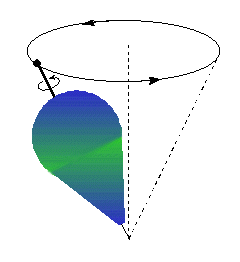
\includegraphics[width=0.5\linewidth]{fig4.png} 
\caption{Precession of the earth's axis pt.1 \\ Image source \cite{precession1}}
\label{fig4}
\end{center}
\end{wrapfigure}
An important point that I would like to add is the concept of \textbf{epoch}, I am not sure how useful this could be for outreach, however, for those of you who are planning to have a career in astrophysics or astronomy would need to know this concept as soon as possible. Now, along with the earth rotating along its rotation axis, and it's revolution around the sun, the earth also precesses around it's rotation axis. Something like that shown in figure \ref{fig4}. The rotation axis rotates around a central axis with a period of $\approx$26000 years (refer \cite{precession1} and \cite{precession3}). Since this happens, over a span of 26000 years, the celestial north pole changes over this time period, since as the axis changes it's direction, so will the north pole change. Right now it is pointing at polaris, however, after $\approx$ 13000 years it would point at the opposite direction nearby Vega, making it our new pole star. 
\paragraph{}
Now, this also means one thing, since the axis changes direction with time, the celestial equator changes as well. This in turn changes the declination and hence the right ascension of the objects. This is a very slow process (a thousand years to see any noticeable changes in the skies) however, when we are doing any deep sky observation, such as trying to communicate the "exact" position of an object, or basic astrometry, we need to be as precise as possible because some of these ra and declination coordinates dictate whether you are looking at one star or it's neighboring star. To eliminate this problem we have the concept of epoch, that is, when we tell someone that this event happened at a certain location, one can point their telescope at that location at that very instant, but then because the earth has precessed away (even if by a very tiny bit), the person might not see the same object, hence we also need to mention when did we observe it so that the person observing could make the necessary calculations to mediate for the earth's precession and hence arrive at the actual object. 
\paragraph{}
\begin{wrapfigure}{l}{0.5\textwidth}
\begin{center}
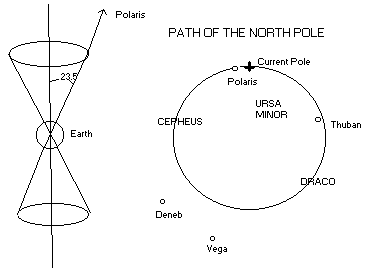
\includegraphics[width=0.8\linewidth]{fig5.png} 
\caption{Precession of the earth's axis pt.2 \\ Image source \cite{precession3}}
\label{fig5}
\end{center}
\end{wrapfigure}
However, this is not enough since with the immense number of observations made on a daily basis, keeping track of those observations and making those calculations is an immense task. Hence we mention certain standardized years when we are mentioning the coordinates, such as J2000, meaning, the coordinate of the object in the Julian year 2000. I would highly recommend one to go through \cite{epoch1}, \cite{epoch2} and \cite{epoch3} for a deeper understanding of the same. The conversions are given in the book \cite{epoch4} (for those who know C++ this book has beautiful codes to do the conversion). 
\paragraph{}
Now, there are several different epochs, and hence when you wish to communicate what you saw, where you saw it, and when you saw it, you need to mention the epoch so that you are able to answer the second question, the first and third being where astrophysics lies and the second is where astrometry lies. \\
\paragraph{}
The figure \ref{fig5} shows the path earth's axis will trace during the $\approx$26000 year cycle. 
\subsection{What are telescopes and how do they work?}
\paragraph{}
A telescope is essentially a light bucket. Imagine the photons to rain down from the heavens all the time, a telescope is a device that harvests this rain of photon and focuses them into a small point so that faint and distant objects are visible to to us. Now, the term telescope is an umbrella term which has many different kind of devices under it, each of them depends on which wavelength you are observing, and what you wish to observe. Recently with the advent of gravitational wave astronomy, a new dimension of astronomy has been introduced. However, since this is at it's infancy, only the future can tell how precise and sensitive it gets.
\paragraph{}
Now, there are a few important concepts that we would have to go through before we can jump into the different kinds of telescopes. 
\begin{enumerate}
\item {\textbf{Mirror assembly and dimensions:} This one of the most important aspect of the telescope. This is what decides what will be seen and what wont, and what kind of "effects" one can expect. Now, based on these there are two major subdivisions of telescopes namely;
\begin{enumerate}
\item \textbf{Refractor Telescopes:} These are the telescopes that work on the principle of refraction. Light is passed through a primary lens of a certain diameter (which is the \textbf{aperture}) and the light is then focused on a point at the rear end of the telescope, where the eyepiece is responsible for further focusing the light into the eye of the observer. 
\item \textbf{Reflector Telescopes: } These kind of telescopes work on the principle of reflection. They too are comprised of a primary mirror, however, this time the mirror is at the end of the optical tube. The diameter of the mirror acts as the aperture, and whatever light falls on it is then focused to a point in front of the telescope, which is then redirected using a secondary mirror into the eyepiece.
\item \textbf{Catadioptric Telescopes: } These are sort of a hybrid telescope that incorporates certain refracting and reflecting components into the telescope optics that helps in the correction of aberrations caused due to one of the components in the optical assembly. 
\paragraph{}
\begin{figure}[h]
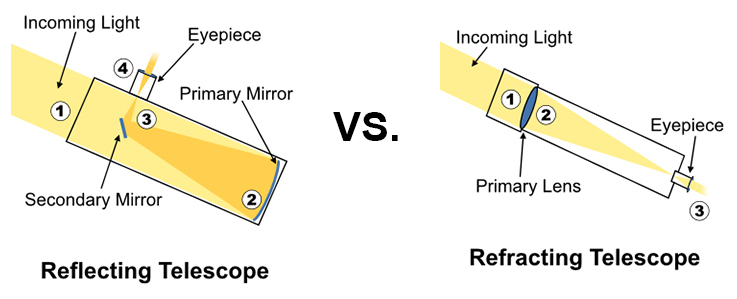
\includegraphics[width=1.0\linewidth]{fig7.jpg}
\caption{Basically this is how the two telescopes work.}
\label{fig7}
\end{figure}
\end{enumerate}
\item \textbf{Mount}: This is the setup on which the telescope stands. Based on their mechanism and how they move about, there are two kinds of telescope mounts;
\begin{enumerate}  
\item \textbf{Equatorial mount:} An Equatorial mount, as mentioned previously, allows observers to follow the rotation of the sky as the Earth turns. The advantageous feature of this mount is its availability to follow any object in the sky without the observer's need to make adjustments on two axes. This is a great help, for example, when on is trying to find their way among the stars with a map. Equatorial mounts are also better options if you do frequent astrophotography. These kind of telescopes also have a lot of scientific application pertaining to the ease of conversion of the coordinates with epochs, and much more. 
\item \textbf{Alt-azimuth mount:} The Alt-azimuth mounts in contrast have a simpler design, meaning they just swing up, down, left and right. You have to move the scope every so often to follow the stars, moons and planets as the earth turns. An alt-azimuth mount is both cheaper and lighter for the same degree of stability but it misses out on the ability to easily follow the rotation of the sky when the earth turns. Dobsonian telescopes function on the Alt-azimuth mount too.
\end{enumerate}
}
\item {\textbf{The auxiliary optics involved:} These encompass things such as: 
\begin{enumerate}
\item \textbf{The eyepiece:} This is responsible for the magnification of the telescope. The relation between the magnification and eyepiece is as follows:
\begin{center}
\begin{equation}
\frac{Telescope \ Focal \ length}{Eyepiece \ Focal \ length} = Magnification
\end{equation}
\end{center}

\item \textbf{The view-finder:} This, in many cases, is a secondary telescope with a much larger field of view which helps the observer to narrow down on the object. The main reason why this is important is because the primary telescope has a very narrow field of view, this makes finding things difficult using the telescope, a collimated (we will come to that later) viewfinder is the key to finding objects efficiently. 

\item \textbf{Optical filters:} They aren't as vital to the functioning of the telescope as the previous two, however, for certain bright objects (and in some cases, deep sky objects), such as moon or sun, they can be comfortably viewed using filters. Filters are extensively used in case of deep-sky astrophotography, or mostly in any and all kinds of scientific measurements. There are different kinds of filters, each of which are tailored to their intended use.  
\end{enumerate}
}
\end{enumerate}
\newpage
\subsection{Telescopes in some detail}
Now, we know the telescopes, and their types, however, let us go a bit deeper into this, know how they work, their underlying principles, etc.
\subsubsection{Reflector Telescopes}
\paragraph{}
\begin{wrapfigure}{l}{0.5\textwidth}
\begin{center}
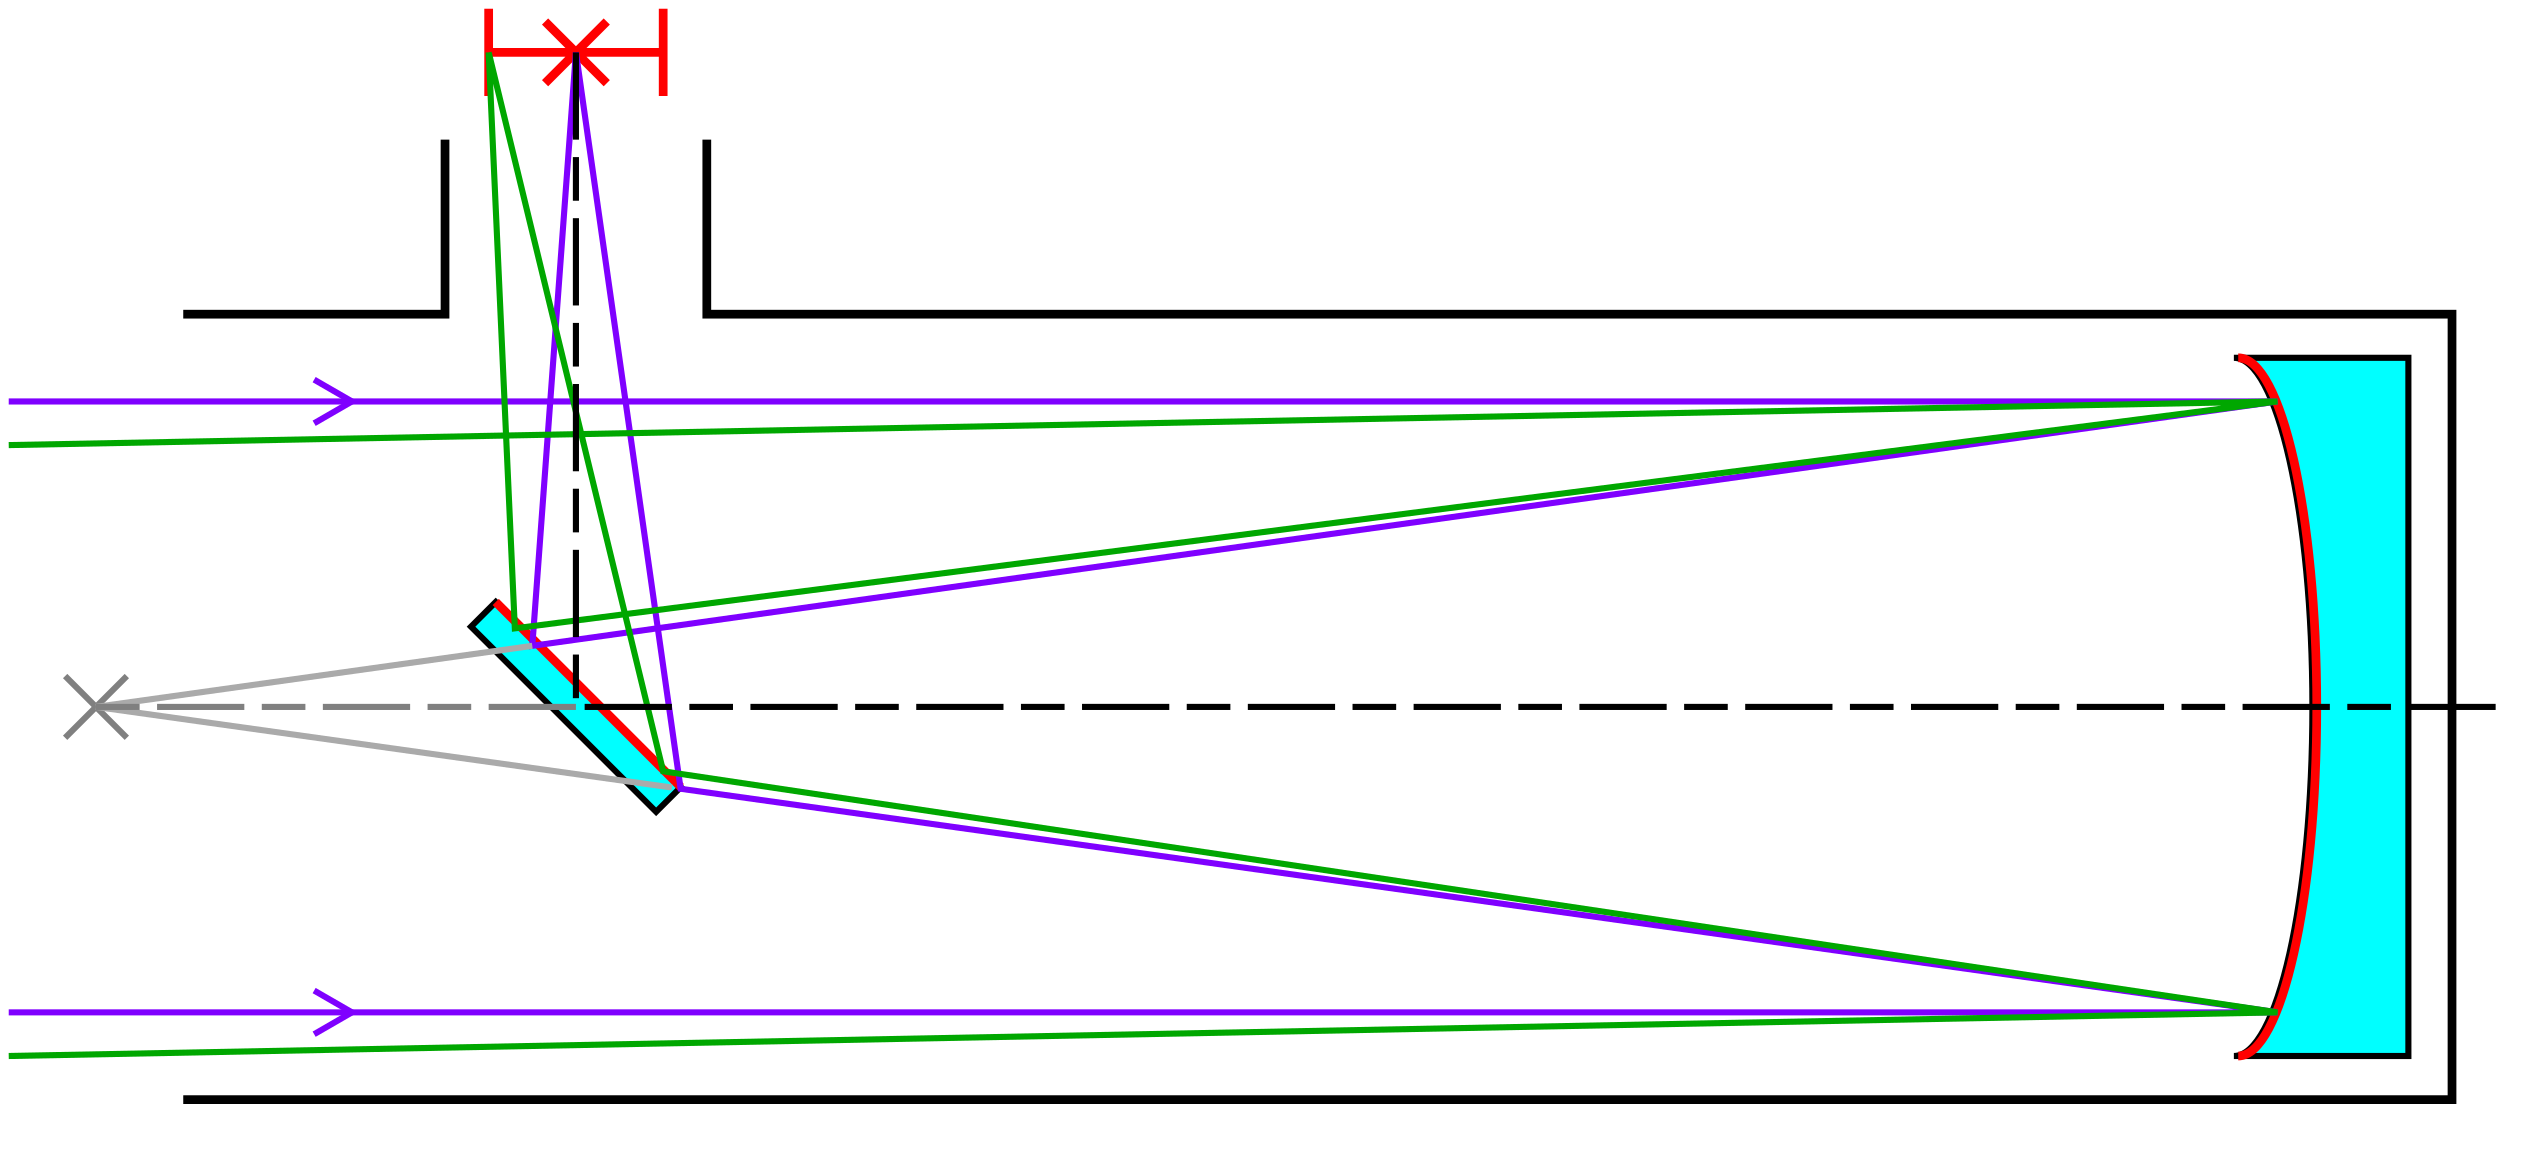
\includegraphics[width=1\linewidth]{fig6.png} 
\caption{Basic design of the Newtonian telescope \\ Image source \cite{newttele2}}
\label{fig6}
\end{center}
\end{wrapfigure}
The most basic design of a reflector telescope could be summarized as a Newtonian telescope. As the name suggests, this was the first successful reflecting telescope, developed by sir Issac Newton in 1668 (\cite{newttele1}), which he built to prove his theory that white light is composed of a spectrum of colors. Now, the concept of the telescope is simple as shown in the figure \ref{fig6}. In the classical sense, the light enters the telescope from the left from infinity, making the beam parallel, it hits the concave mirror at the base of the telescope, which then reflects the light to a plane secondary mirror, which then reflects the beam to the eyepiece. Within the figure \ref{fig6} one would notice that their are two beams, these are to show how the telescope differentiates between two sources in the same field of view (that is, the part of the sky visible through the telescope).
\paragraph{}
Now, as mentioned in the previous paragraph, the two beams represent light coming from two different sources. Now, the two questions that can arise here, (which applies to all kinds of telescopes) would be;
\begin{enumerate}
\item How far apart can these objects be to be visible in the same field of the telescope, and 
\item How close can the two objects be for the telescope to be able to differentiate between the two (so that both of them don't appear as one blob instead of two different blobs).
\end{enumerate}
\paragraph{}
The first question is asking about the field of view of the telescope. There is a very simple formula to calculate the FOV of a telescope;
\begin{equation}
Total \ Field \ of \ View = \frac{Eyepiece \ Apparent \ Field \ of \ View}{Magnification}
\end{equation}
This equation shows us the relation between the field of view and the magnification of the eyepiece/telescope. This also shows that if we know the magnification of the telescope/eyepiece, we can say whether a given object would be visible in it's entirety through the telescope using an eyepiece or not.
\paragraph{}
The second question touches on the concept of \textit{\textbf{angular resolution}}. This is a crucial concept while determining whether a telescope will be able to resolve two extremely close objects or not. This parameter is very sensitive to atmospheric distortions as well. In fact, the angular resolution of a telescope is limited primarily by the atmosphere, one of the reasons why people prefer sending optical telescopes to space. There are work around to these as well, things such as Adaptive Optics (which one can read about in detail in their Wikipedia page \cite{AO1}). This technology helps ground based telescopes to account for the atmospheric jitters that limits the angular resolution. Also note that this is where we insert a bit of physics since the angular resolution depends on the wavelength of the incoming light and the diameter of the telescope. The relation is as follows;
\begin{equation}
Angular \ Resolution \ = 1.22 \times \frac{Wavelength}{Aperture}
\end{equation}
\paragraph{}
Now, the pleasure of finding out how and why this equation came up is something I would leave to you. This equation applies to almost all wavelengths, however, it falls short when the wavelength becomes so small (meaning, the energy of the photon is high, i.e. frequency is high) that it doesn't even interact with the mirror. 
\subsubsection{Refractor Telescopes}
\paragraph{}
These are the kind of telescopes that work on the principle of refraction. These essentially include a primary lens, which focuses the light in towards the eyepiece towards the end of the telescope, as shown in the figure \ref{fig6}. These types of telescope were the first ones to be invented, back in 1608 in the Netherlands by Hans Lippershey and Zacharias Janssen who were spectacle-makers in Middelburg, and Jacob Metius of Alkmaar \cite{Refractor1}. As mentioned in the previous paragraph, Galileo was the first person to have found an alternate use of the refractor telescope. 
\paragraph{}
There were several design improvements to the Galilean refractor telescope. Improvements such as the \textbf{Keplerian telescope}, which replaced the concave eyepiece with a convex eyepiece which reduced the strain on the eyes while looking at an object. This however had the image inverted and required precise optics to counter one of the biggest problems with refractor telescopes, \textbf{chromatic aberration}. Another kind of refractors are the \textbf{Achromatic refractors} and the \textbf{Apochromatic refractors}.
\subsubsection{Catadioptric Telescopes}
\paragraph{}
Now we have refractors that are made up of lenses, and we have reflectors that are made up of mirrors. So logically, one might ask, what if you combine them to make a third category of telescopes. The result of such a combination would be the Catadioptric Telescopes. These generally have a primary mirror paired with a a thin lens/mirror, generally called a corrector lenses which is responsible for correcting any minor aberrations caused due to any other element in the optical setup. Also because of the way the light is redirected within the telescope, the telescope can be relatively smaller and easier to make, since now, because of the corrector optics, one can achieve relatively higher optical quality using many mediocre optical components, each working to counteract the aberrations caused due to each other, resulting in a sharp wide-field image. 
\subsection{Why are reflectors preferred over refractors?}
\paragraph{}
There are several reasons why reflectors are preferred over refractors. Some of them are: 
\begin{enumerate}
\item {\textbf{Minimal chromatic aberration:} Chromatic aberration is what we see as rainbow effects around the edges on an object. This effect is generally seen when the light is not focused properly on the focal plane. One of the many reasons why focusing white light isn't so easy is because of the intrinsic nature of light and it's wavelength, that is, how red wavelength bends much less than blue. This difference causes red and blue wavelengths to focus at different points and hence one way observe the edges of an image formed at the focal plane to appear distorted. A good example of the same would be to look at images from high quality lenses and comparing the same with that of low quality lenses. This kind of image distortion causes problems with spectroscopy and classification of the star. 
\\ The reason why reflectors do not suffer from such kind of distortion is because the light does not pass through any lens in the first place. That is, the light is reflected from mirrors to other mirrors and is finally focused on a focal plane. Since the light does not have to pass through any kind of material, there is no chromatic aberration. Apart from this, the refractor would be much more prone to another kind of aberration called the spherical aberration. This is the kind of aberration that is caused due to minor inaccuracies in curvature of the mirror/lens. Both reflectors and refractors suffer from this kind of aberration. 
}
\item {\textbf{Refractors are bulky:} Refractors require relatively bulky optics in order to make a telescope with comparable performance to a much lighter reflector. Given the lens requirements, reflectors are inherently bulky and hence require much more efforts to make, maintain, slew and track.
}
\end{enumerate}
\paragraph{}
Given the viability of reflectors, one can imagine why there are so many different kinds of reflector telescopes. These are all made in order to improve upon the previous generation's errors. And now, with the advent of Catadioptric telescopes, one can obtain greater angular resolution than what was previously achievable. 

\subsection{The "Glass Ceiling" for a telescope.}
\paragraph{}
Now, assume that we have a telescope that has a high angular resolution, so high that, on paper it can see a star as it is, that is, a point source of light. However, on earth, because of our atmosphere, and the thermal jitters in the atmosphere, the net "image" that we get is always a blurred version of that point source. This causes the image of the star to seem out of focus and hence creates problems with larger telescopes that are, on paper, are able to resolve very fine features, but are unable to do so because of the atmospheric effects. One can see that because of this, any telescope larger than 10 inches (primary mirror diameter) would be useless for high precision photometry because of the atmospheric jitters.
\paragraph{}
This is where the concept of \textbf{Adaptive Optics} comes in. The name suggests that it is a technique that adapts to the minute changes in the atmosphere, things such as turbulence, and hence nullifies their effect. The way this is achieved is interesting and hence I would urge you to read through \cite{AO1}, \cite{AO2} and \cite{AO3}, and many more to gain a deeper understanding of the concept. 
\paragraph{}
In order to nullify the atmospheric effects, AO systems pick a guide star (this is a star that has a well known spectrum, and lies in the same field of view as the observed abject), or create an artificial star using LASERs. Then it observes the light from that star and see what variations the atmosphere imparts on the light. And now since the phase of the initial light is known, they simply alter the mirror dimensions to counteract the phase differences imparted due to the atmosphere. A fun experiment would be to use the equation for angular resolution and find out the maximum mirror diameter beyond which one would have to use AO to make the best possible use of it.
\subsection{How do we measure distances is astronomy?}
\paragraph{}
This is what is called the distance ladder is astronomy. This is called so because there is no standard way of measuring distances in astronomy given the immense distances to the stars and galaxies. The distance ladder goes as follows:
\begin{enumerate}
    \item \textbf{Distance in terms of Astronomical Units (AU)}: An astronomical unit is the distance between the earth and sun. This is approximately 1.4959 $\times$ 10$^{11}$ m or 149597870700 m (exactly). This is used as the basic distance measurement unit since one cannot use standard units such as km or miles in order to measure distance to the stars. 
\end{enumerate}




\newpage
\clearpage
\begin{thebibliography}{20}
\bibitem{Planets_1}
Bryner, Jeanna. “The Storied History of the Word 'Planet'.” Space.com, Space.com, 8 Mar. 2016, www.space.com/5743-storied-history-word-planet.html.

\bibitem{wiki_planet_round}
Wikipedia contributors. "Spherical Earth." Wikipedia, The Free Encyclopedia. Wikipedia, The Free Encyclopedia, 22 Aug. 2018. Web. 23 Aug. 2018.

\bibitem{OTSOG}
Hawking, Stephen. On the Shoulders of Giants: the Great Works of Physics and Astronomy. Running Press, 2002.

\bibitem{AASP}
Strous, Louis. “Ask A Solar Physicist FAQs - Answer.” Stanford Solar Center, solar-center.stanford.edu/FAQ/Qsunasstar.html.

\bibitem{ASHistory}
“Spectroscopy and the Birth of Astrophysics (Cosmology: Tools).” The Discovery of Global Warming - A History, Center for History of Physics, history.aip.org/exhibits/cosmology/tools/tools-spectroscopy.htm

\bibitem{wiki_constellation}
Wikipedia contributors. "Constellation." Wikipedia, The Free Encyclopedia. Wikipedia, The Free Encyclopedia, 19 Aug. 2018. Web. 25 Aug. 2018.

\bibitem{constellationsHist}
Rao, Joe. “How the Night Sky Constellations Got Their Names.” Space.com, Space.com, 8 Mar. 2016, www.space.com/15486-night-sky-constellations-names.html.

\bibitem{astrometry_wiki}
Wikipedia contributors. "Astrometry." Wikipedia, The Free Encyclopedia. Wikipedia, The Free Encyclopedia, 21 Aug. 2018. Web. 25 Aug. 2018.

\bibitem{azimuth_wiki}
Wikipedia contributors. "Azimuth." Wikipedia, The Free Encyclopedia. Wikipedia, The Free Encyclopedia, 27 Jul. 2018. Web. 26 Aug. 2018.

\bibitem{coord_wiki}
Wikipedia contributors. "Celestial coordinate system." Wikipedia, The Free Encyclopedia. Wikipedia, The Free Encyclopedia, 20 Aug. 2018. Web. 26 Aug. 2018.

\bibitem{equi_coord1}
“Equatorial Coordinate System | COSMOS.” 7, astronomy.swin.edu.au/cosmos/E/Equatorial Coordinate System.

\bibitem{equi_coord2}
“Celestial Coordinate System.” Classification of the Planets, \\www.pas.rochester.edu/~blackman/ast104/coordinates.html.

\bibitem{precession1}
“The Precession of the Earth's Axis.” Structure of a Black Hole, \\astrosun2.astro.cornell.edu/academics/courses/astro201/earth\_precess.htm.

\bibitem{precession2}
“The Earth's Wobble – Precession.” My Dark Sky, 14 Oct. 2008, mydarksky.org/2008/10/14/the-earths-wobble-precession/.

\bibitem{precession3}
“Astronomy: Precession of Earth.” Astronomy: Greek Astronomy, astro.wsu.edu/worthey/astro/html/lec-precession.html.

\bibitem{epoch1}
Wikipedia contributors. "Epoch (astronomy)." Wikipedia, The Free Encyclopedia. Wikipedia, The Free Encyclopedia, 6 Aug. 2018. Web. 30 Aug. 2018.

\bibitem{epoch2}
Wilkins, D.R., and S.J. Crass. “J1950 And J2000 Epochs.” Stellar Mass and Supermassive Black Holes | Institute of Astronomy, Institute of Astronomy , www.ast.cam.ac.uk/public/ask/1960.

\bibitem{epoch3}
“Epoch | COSMOS.” 7, astronomy.swin.edu.au/cosmos/e/epoch.

\bibitem{epoch4}
Montenbruck, Oliver, and Thomas Pfleger. Astronomy on the Personal Computer. Springer Verlag, 2013.

\bibitem{newttele1}
Hall, Alfred Rupert. Isaac Newton: Adventurer in Thought. Univ. Press, 2000.

\bibitem{newttele2}
Wikipedia contributors. "Newtonian telescope." Wikipedia, The Free Encyclopedia. Wikipedia, The Free Encyclopedia, 28 Jul. 2018. Web. 30 Aug. 2018.

\bibitem{Tele_form1}
Chuck Hawks. “Simple Formulas for the Telescope Owner.” Sky \& Telescope, 20 Nov. 2017, www.skyandtelescope.com/observing/stargazers-corner/simple-formulas-for-the-telescope-owner/.

\bibitem{TeleFOV}
Swanson, Mike. “Field of View in a Telescope.” Nexstarsite, Ryukyu Astronomy Club, www.nexstarsite.com/\_RAC/articles/fieldofview.htm.

\bibitem{AO1}
Wikipedia contributors. "Adaptive optics." Wikipedia, The Free Encyclopedia. Wikipedia, The Free Encyclopedia, 20 Jun. 2018. Web. 26 Sep. 2018.

\bibitem{Refractor1}
Wikipedia contributors. "Refracting telescope." Wikipedia, The Free Encyclopedia. Wikipedia, The Free Encyclopedia, 14 Sep. 2018. Web. 26 Sep. 2018.

\bibitem{ChromatAberration}
Wikipedia contributors. "Chromatic aberration." Wikipedia, The Free Encyclopedia. Wikipedia, The Free Encyclopedia, 25 Apr. 2018. Web. 1 Oct. 2018.

\bibitem{CataTele}
Wikipedia contributors. "Catadioptric system." Wikipedia, The Free Encyclopedia. Wikipedia, The Free Encyclopedia, 9 Jul. 2018. Web. 10 Oct. 2018.

\bibitem{AO1}
Wikipedia contributors. "Adaptive optics." Wikipedia, The Free Encyclopedia. Wikipedia, The Free Encyclopedia, 2 Oct. 2018. Web. 10 Oct. 2018.

\bibitem{AO2}
information@eso.org. “Adaptive Optics.” ESO, www.eso.org/public/teles-instr/technology/adaptive\_optics/. 

\bibitem{AO3}
Sky $\&$ Telescope. “Adaptive Optics: Before and After.” Sky $\&$ Telescope, Sky $\&$ Telescope, 21 Mar. 2016, www.skyandtelescope.com/sky-and-telescope-magazine/beyond-the-printed-page/adaptive-optics-before-and-after/.

\end{thebibliography}
\end{document}

